\section{Method}

\subsection{Data preprocessing}
Starfish text content is serialized as HTML, a format which is not suitable for calculating semantical similarity. Before processing, the data is sanitized by removing HTML tags and entities and convert unicode characters to their closest ASCII representation.

Maybe something about creating the folds by removing some of the documents?

\subsection{Text descriptors}
\subsubsection{Textvectorizer}

The first set of vectorizers focuses on the texts of the documents. The \emph{textvectorizer} is a very generic approach that can be used on any corpus of textual documents. In the Starfish context, we define 'content' as the title and text-fields of a document. The only exception on this are Persons, of which we wil use the name and about-fields. 

The textvectorizer first transforms the set of documents into a bag of words and calculates the TF-IDF values for all words. This was done using the TFIDFVectorizer of scikitlearn \citep{scikit-learn}.  Though the TF-IDF values of words that are used very often should be low, common words such as 'and', 'or' and 'of' are still present in the vectors. This could be caused by the different types of documents. For example, a Question often structured in a less complex way than a Project description. To prevent this from happening, the English stopword list that comes standard with scikit learn was used to remove these words from the document descriptors.

\subsubsection{Weighted textvectorizer}
The weighted text vectorizer is an extension of the textvectorizer that takes into account the links of the proposed documents. The vectors of the links of a document are added with some weight to the vectors of the documents themselves. Intuitively, this would add semantic information about a document based on it's links. For example, a Person is likely to write other documents about his or her subjects of expertise. Knowing not only the biography of a Person, but also the content he or she has added to Starfish, gives a more complete image of what documents could be related to that Person.

The vectors of links of a document are added in a recursive way, where documents that are linked directly have a higher weight than documents that are linked transitively. The algorithm is displayed in figure xx.

\subsection{Tag descriptors}
\subsubsection{Simple tag vectorizer}
The tag-based approach is more Starfish specific than the text-based approach, since it depends on the tags that are available in Starfish. The tags on Starfish are added by the users themselves, so offer a human-based vision on what a document is really about. The simple tag vectorizer is a very straight forward implementation of the idea of using tags. The vectors of this transformation consist of a binary list that tells whether or not a tag is attached to the document. 

\subsubsection{Tag smoothing}
The tag smoothing vectorizers creates descriptors based on the tag set of a document. A tag co-occurs with other tags in a document, we assume documents with similar tags should be linked in Starfish. Let the frequency of occurrence with other tags across the dataset will form a vector for each tag. The descriptor for a document is then created by combining the occurrence vectors for all the document's tags. Now documents with tags that occur together will be seen as similar.

There are two reasons why one would like to smooth the tag co-occurences. Firstly, a problem for this is that tags must occur together before the algorithms works properly. The Starfish dataset contains a lot of tags that only occur with a small frequency, which means the tag occurrence vector will contain many zeros. This makes the algorithm perform bad with little data. Secondly, two tags can describe the same concept and be connected to that concept through a common co-occurence with another tag. Whilst they describe the same concept and are connected to that, they are not directly linked together. Therefore it seems feasible to perform some sort of smoothing on the co-occurences of tags.

\citet{zhou2011web} proposed a method to cluster web documents based on tag set similarity. This is based on a similarity between two tags as a relation between the frequency these tags occur separate and together, as described in equation~\ref{eq:tag_similarity}. To smooth these similarities between tags, a tag similarity matrix $\mathcal{C}$ is constructed. Each entry $c_{i,j}$ in this matrix can be viewed as the angle $\theta_{i,j}$ between two unknown vectors $v_i$ and $v_j$. These vectors cover both explicit similarity and implicit similarity \citep{park2010vector}. This transfers the problem to find a set of linearly independent vectors $\{v_1,v_2,\ldots,v_n\}$ for which for all $v_i \cdot v_j = \cos(\theta_{i,j})$. One must find a matrix $\mathcal{V}$ for which $V^TV = C$. This can be done by orthogonal triangularization on $\mathcal{C}$ for which \citeauthor{zhou2011web} introduces a modified Cholesky transform.

\begin{equation} \label{eq:tag_similarity}
s_{i,j} = \frac{f_{i,j}}{f_i + f_j - f_{i,j}}
\end{equation}


\subsubsection{Glossaries of tags}
The glossaries of tags approach is also based on the intuition certain tags cover overlapping concepts, something which is not always directly reflected by tag frequencies. In the Starfish system, a tag is expected to have a glossary; a short English description of the concept a tag. If tags are related then the glossaries of those will contain terms and words more similar to each other than to other tags' glossaries. The glossaries of tags approach aims to use the network between, visible through glossary similarity, to calculate document similarity.
The vectorizer creates a document descriptor based on the bag of words model for all glossaries. Each tag with a glossary is transformed into a vector using TF-IDF, these vectors are then summed to create the descriptor for a document.

\subsubsection{Weighted tag vectorizer}
The weighted tag vectorizer uses the same method as the glossaries of tags vectorizer, except the tag vectors are summed with a weight proportionally to the inverse tag frequency instead of equally. Tag descriptors for infrequent tags have more influence on this descriptor.

\subsection{Distance metrics}
Short description of how these were implemented

\subsection{Bayesian weighting}
Explain motivation, theory and implementation 

\subsection{Thresholds}
After creating the descriptors for a document and finding a new document's nearest neighbors, a subpart of those links needs to be returned by the linker application. An average document in Starfish has x links. To create a dynamic threshold which returns similar a similar amount of documents, a document from the Starfish data is extracted and then to re-inserted to test the number of links the system returns to the number of links the document had in the original system. Figure~\ref{fig:link_histogram} shows the distribution of outgoing links in the current network.

\begin{figure}[h]
\centering
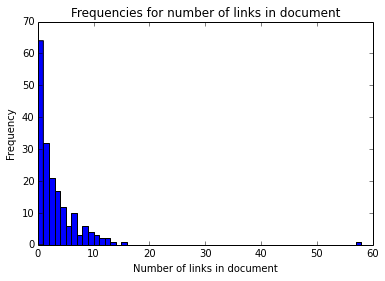
\includegraphics[width =0.45\textwidth]{images/link_histogram}
\caption{The frequency of outgoing links in Starfish documents}
\label{fig:link_histogram}
\end{figure}

In figure~\ref{fig:thresholds}, the distances for nearby documents the system recommends can be viewed. On the horizontal axis, the documents are shown in sorted order. The vertical axis displays the cosine distance for that document has from the new document. The patterns for all vectorizers seem very noisy, especially for documents that had very little links in the original document. The documents which had more links in the original dataset seem to be less scattered and more plausible to fit to a line.

\begin{figure}[h]
\subfigure[Weighted tags]{	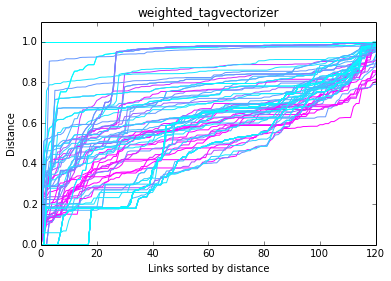
\includegraphics[width =0.24\textwidth]{images/threshold_weighted_tag}	}
\subfigure[text]{				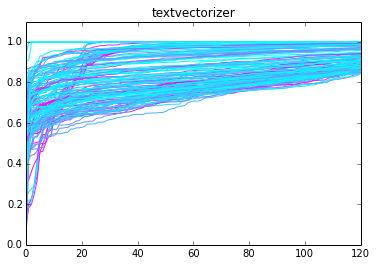
\includegraphics[width =0.24\textwidth]{images/threshold_text} 			}
\subfigure[tag smoothing]{	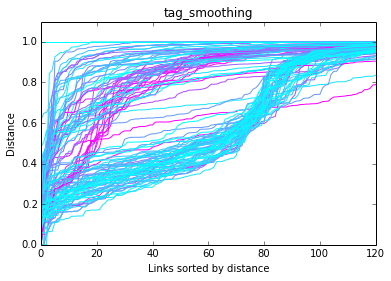
\includegraphics[width =0.24\textwidth]{images/threshold_smoothing} 		}
\subfigure[glossaries]{		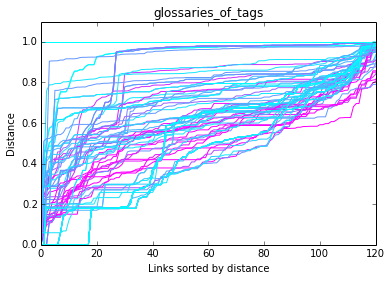
\includegraphics[width =0.24\textwidth]{images/threshold_glossary} 		}
\caption{The blue purple gradient represents documents with 0 links (blue) to >10 links (purple)}
\label{fig:thresholds}
\end{figure}

The the threshold should depend on multiple factors which mostly depend on the setting in which the document linker will be used. Two major factors determine how the threshold should work.
\begin{enumerate}[1.]
	\item The degree of certainty we expect from the returned documents.
	\item The maximum number of documents that should be returned for a specific application.
\end{enumerate}
If the system is used to directly create the links into the Starfish system, the first aspect is very important. Only documents with a very high degree of linking certainty should then be returned, the amount should be based on the contents of the current system. If the system will be used to create recommendations which a user must accept or reject, the first aspect becomes less important and the system should return an amount of links which can quickly be reviewed by users. To ensure the flexibility for choice of algorithm and integration of the application, the threshold algorithm will contain a configurable parameter.

\begin{figure}[h]
\subfigure[Weighted tags]{	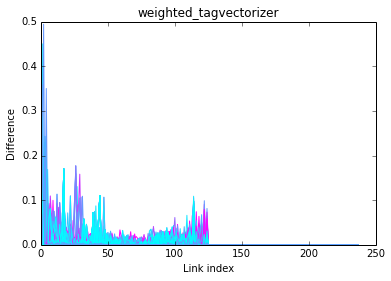
\includegraphics[width =0.24\textwidth]{images/threshold_weighted_tag_difference}		}
\subfigure[text]{				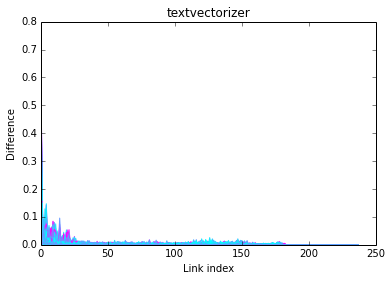
\includegraphics[width =0.24\textwidth]{images/threshold_text_difference} 			}
\subfigure[tag smoothing]{	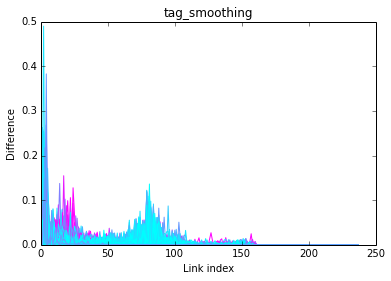
\includegraphics[width =0.24\textwidth]{images/threshold_smoothing_difference} 		}
\subfigure[glossaries]{		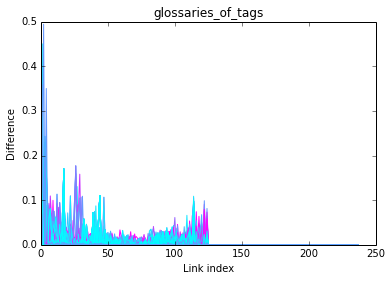
\includegraphics[width =0.24\textwidth]{images/threshold_glossary_difference} 		}
\caption{Distance betweeen two nearest neighbors}
\label{fig:thresholds_differences}
\end{figure}

When adding a document to Starfish, it is assumed that there is always at least one related document. Based on the distance of the nearest neighbor for the new document, the index of a and the configurable parameter, the threshold is defined as in equation~\ref{eq:thresh}. In this equation, $\alpha$ is the configurable parameter, $m$ is the number of documents returned by the nearest neighbor algorithm, $d_0$ is the distance to the closest document, $\frac{m - n}{m}$ is a factor that ensures the maximum allowed distance decreases for documents ranked further away. This is based on the differences between two nearest neighbors which are visualized in figure~\ref{fig:thresholds_differences}. The distances have a long tail form: the distances between the nearest neighbors is relatively large for the closest documents and smaller between the documents further away. 

\begin{equation}
t_n = \alpha (1 - d_0) \frac{m - n}{m}
\label{eq:thresh}
\end{equation}